\scanpage{27}
% archive sheet number: 26

this last relation $\Sigma_1^-\cap\Sigma_2^-\ne\varnothing$ is true
$=$ if $E_1=E_2=\varnothing$, for
\deleted{\unsure{therefore|then} by hypothesis} if we also had
$\Sigma_1^-\cap\Sigma_2^-=\varnothing$, we would conclude from this that the two
\deleted{partitions} binary decompositions \deleted{\unsure{its|are|themselves}}
(which are then binary partitions) are \uline{identical},
which we \inserted{have} excluded. This shows that the
$\Sigma_1^+,\Sigma_2^+$ are uniquely determined.

We thus have the diagram of inclusions
\diagram{\begin{tikzcd}[ampersand replacement=\&,column sep=small]
\Sigma_1^+ \& E_1 \arrow[l,hook] \arrow[r,hook] \& \Sigma_{12}
\& E_2 \arrow[l,hook] \arrow[r,hook] \& \Sigma_2^+
\end{tikzcd}}
which we, express by a diagram
\figure{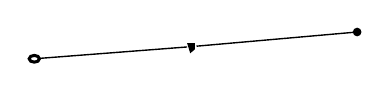
\begin{tikzpicture}[x=1cm,y=1cm]
\draw[line width=0.5pt] (0,0) -- (1.94,0.15);
\draw[line width=0.5pt] (2.06,0.16) -- (4.10,0.34);
\draw[fill=white,line width=1.1pt] (0,0) ellipse[x radius=0.065,y radius=0.043];
\fill (1.94,0.20) -- (2.04,0.20) -- (2.04,0.12) -- (1.98,0.07) -- cycle;
\fill (4.10,0.34) circle[radius=0.055];
\end{tikzpicture}}
\diagram{\begin{tikzcd}[ampersand replacement=\&,column sep=small]
\Sigma_1^+ \& E_1 \arrow[l,hook] \arrow[r,hook] \& \Sigma_{12}
\& E_2 \arrow[l,hook] \arrow[r,hook] \& \Sigma_2^+
\end{tikzcd}}

\margin{\[
\text{NB}\left\{\begin{aligned}
\Sigma_1^-&=\Sigma_{12}\amalg_{E_2}\Sigma_2^+\\
\Sigma_{\deleted{\unsure{1}}2}^-&=\deleted{E}\Sigma_{12}\amalg_{E_1}\Sigma_1^+
\end{aligned}\right.
\]}

% slanted
\margin{This does not imply that the four sets
$\Sigma_1^+,\Sigma_1^-,\Sigma_2^+,\Sigma_2^-$ are distinct,
for we can have (\unsure{indeed not|not} $\Sigma_1^+=\Sigma_2^+$,
nor $\Sigma_1^-=\Sigma_2^-$, but) $\Sigma_1^+=\Sigma_2^-$,
which is equivalent to $E_1=\Sigma_{12}$ and implies $E_2=\varnothing$
(\unsure{this|This} means, in terms of the $(\Sigma_{\unsure{1|t}}^+,\Sigma_1^-)$ that
$\Sigma_2^{\unsure{\dot{-}|-}}=\Sigma_1^+$,
$\Sigma_2^+=X\setminus\Sigma_1^+=\overset{\leftarrow}{\Sigma}{}_1^{-,\unsure{\circ|0}}$)
\deleted{\unsure{or}} and the \unsure{symmetric|symmetric} relation.
We do not want to exclude this case, i.e.\ \deleted{\unsure{we|but}}
do not require that the four sets
$\Sigma_1^+,\Sigma_1^-,\Sigma_2^+,\Sigma_2^-$ be distinct
if they \unsure{\deleted{are}|are}, we say that the
\deleted{sets} \inserted{two binary decompositions}
\deleted{\unsure{are strictly|are strictly}} non-parallel.}

I propose to study the finite
\unsure{indexed|indexed} sets
$\deleted{\unsure{\Pi|\Sigma}}(\unsure{\Pi|\pi}_\alpha)_{\alpha\in A}
\deleted{=(\unsure{\Sigma_\alpha^i}),\unsure{\alpha\in A}}$
$\deleted{\Pi_\alpha=\{\Sigma_\alpha^\varepsilon}$
of binary decompositions of $\unsure{X}$ pairwise non-parallel.

Here is a very \unsure{general|general} way
of obtaining \unsure{heaps|heaps} \deleted{of them}.
